\section{延迟的性质}
\label{sec:nature_delays}

从\gls{dmdp}的通用定义出发，可以研究许多子情形。
本节旨在给出文献或实际\gls{rl}应用中遇到的延迟类型概览。首先介绍定义延迟的不同属性。
最后给出本论文关于延迟的假设。

\begin{figure}[t]
    \centering
    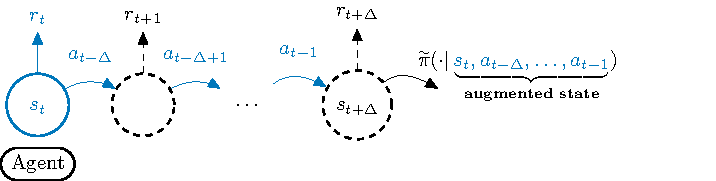
\includegraphics[bylabel=undelayedmdp]{img/thesis_plots.pdf}
    \caption{无延迟\gls{mdp}的表示。}
    \label{fig:undelayed_mdp}
\end{figure}

\subsection{常值延迟与随机延迟}
\label{subsec:constant_stoch_delays}
如前所述，延迟是随机变量，但文献中通常假设常值延迟（constant delay）。
这一简化模型对许多应用而言已足够现实，尤其是当延迟的潜在随机性相对于过程步长可忽略不计时。
例如，\cite{ramstedt2019real}在自动驾驶仿真和连续机器人运动控制中考虑1步常值延迟；\cite{hester2013texplore}在自动驾驶中考虑2步延迟；\cite{walsh2009learning}在简单仿真任务（包括网格世界）中考虑1到20之间的各种延迟。
在主动流动控制中，延迟甚至可达63步\cite{mao2022active}。
然而，对于某些应用，必须对延迟的随机性进行建模。
在\cite{bouteiller2020reinforcement}中，随机延迟（stochastic delay）由策略通过WiFi传输至飞行机器人以及观测数据回传所引起。
\cite{campbell2016multiple}研究了泊松分布延迟对Q学习的影响。
总的来说，即使实际延迟通常非常值，假设常值延迟是为了简化问题，前提是延迟的变化对模型性能不关键。

\subsection{状态观测延迟与动作执行延迟}
\label{subsec:state_action_delays}
当智能体无法获知当前状态但能访问\gls{mdp}的历史状态时，即出现状态观测延迟（state observation delay）。
这与\gls{pomdp}形成对比：在\gls{pomdp}中，历史状态通常不向智能体公开，而是揭示关于当前状态的某些部分信息。\Cref{fig:state_obs_delayed_mdp}展示了状态观测延迟的示例，与之对比的是\Cref{fig:undelayed_mdp}中的无延迟\gls{mdp}。
在图示中，读者可能注意到增广状态（augmented state）这一概念，即最后观测到的状态$s_{t-\delay}$与智能体在过去已选择但尚未观测到结果的所有动作$a_{t-\delay},\dots,a_{t-1}$的拼接。
这一概念是延迟强化学习的核心。
实际上，通过考虑增广状态，智能体汇集了关于延迟过程的所有可能信息。
在马尔可夫性质下，考虑比$s_{t-\delay}$和$a_{t-\delay}$更早的状态或动作将是冗余的。

动作执行延迟（action execution delay）发生在智能体虽然观测到当前状态，但选择的动作将在未来若干步之后才执行的情况。
\Cref{fig:action_exec_delayed_mdp}展示了动作执行延迟的示例。
注意此情形下增广状态的定义。
与状态观测延迟类似，增广状态穷尽描述了延迟环境。
另一个有趣之处在于时间索引。
对于动作执行延迟，智能体在时间$t$选择的动作记为$a_t$。
由于延迟，该动作将在时间$t+\delay$施加于状态$s_{t+\delay}$。
这与状态观测延迟形成对比：在状态观测延迟中，智能体在时间$t$选择的动作$a_t$将施加于当前未观测的状态$s_t$。
对于常值延迟，可以将动作索引偏移$\delay$，使得动作$a_t$如无延迟\gls{mdp}那样施加于$s_t$。
但这仅对常值延迟\gls{mdp}可行。
若延迟为随机，则智能体在时间$t$选择的动作标签将是随机的。
此外，若两个动作因随机延迟同时施加，它们将被赋予相同索引。
这似乎不是良好的命名方式。
因此，无论在何种情形下，本文使用智能体选择动作的时间作为该动作的索引。
该记号的另一优势在于，如\Cref{fig:state_obs_delayed_mdp}和\Cref{fig:action_exec_delayed_mdp}所示，状态观测延迟和动作执行延迟的增广状态相同。

\begin{figure}[t]
    \centering
    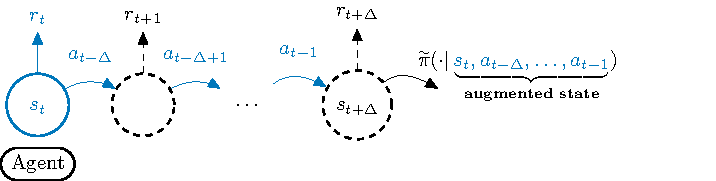
\includegraphics[bylabel=stateobsdelayedmdp]{img/thesis_plots.pdf}
    \caption{具有状态观测延迟的\gls{dmdp}的表示。}
    \label{fig:state_obs_delayed_mdp}
\end{figure}

\begin{figure}[t]
    \centering
    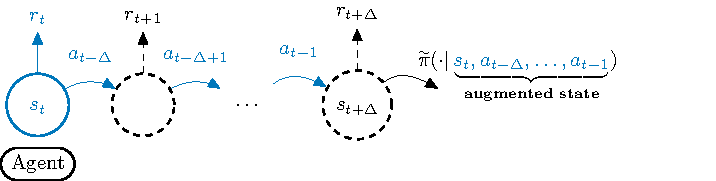
\includegraphics[bylabel=actionexecdelayedmdp]{img/thesis_plots.pdf}
    \caption{具有动作执行延迟的\gls{dmdp}的表示。}
    \label{fig:action_exec_delayed_mdp}
\end{figure}

后文将看到，动作执行延迟和状态观测延迟是等价的，其效应可叠加（\Cref{subsubsec:equiv_action_state_delays}）。
因此，在上图中刻意以类似方式表示这两类延迟。
其增广状态遵循相似构造，且对于相同延迟量包含相同数量的项。
然而，如下文所述，存在一些微小差异，但只要避免混淆就不影响理论分析。
正如\cite{chen2021delay}所指出的，动作执行延迟可能引起一个小问题：延迟可分为两部分——动作选择和动作执行。
前者是智能体在观测到最新状态后计算动作所需的时间。
后者是智能体在环境中实际执行该动作所需的时间。
后者来源是传统意义上的动作执行延迟，而前者来源在实践中可能造成问题。
实际上，若环境在智能体仍在计算前一个动作时提供了新状态（即动作选择延迟长于环境步长），则智能体尚不知晓其前一个动作。
这对之前介绍的增广方法构成问题，我们将在\Cref{sec:related_works}中详细讨论。
这些方法基于先前动作选择当前动作。
因此，此处先前动作集合中缺失了一个动作。
智能体可等待后再计算下一个动作，但延迟将累积，缺失动作的数量会增加。
为避免此类情况，如\cite{chen2021delay}所述，本文假设动作选择延迟小于\gls{mdp}步长\footnote{若实践中不满足此条件，可将动作持续多个步长，以人工创建步长更长的\gls{mdp}，如\cite{metelli2020control}中所述。}。
状态延迟与动作延迟的另一个区别在于奖励收集延迟对二者的影响。
如\cite{katsikopoulos2003markov}所述，在状态观测延迟情形下，若无奖励延迟，智能体观测到与当前未观测状态相关的随机变量的结果。
事实上，当前奖励是当前未观测状态的函数。
换言之，该设置提供了关于当前未观测状态的部分信息。
相反，在动作执行延迟情形下，无奖励延迟不会向智能体提供额外信息，因为最新信息（当前状态）已经是已知的。

\subsection{奖励收集延迟}
\label{subsec:reward_delay}
此处可能需要澄清。
在\gls{rl}文献中，两类不同但相关的问题都可能被称为延迟奖励（delayed reward）。
在许多实际问题中，定义每步奖励可能很困难，而将全部奖励集中到单个步骤中则更容易\cite{han2022off}。
例如，在棋类比赛中为每一步设计奖励很困难，而根据比赛结果给予0或1的奖励则简单得多。
这是第一类延迟奖励，也称为稀疏奖励（sparse reward）。
它通常涉及\gls{mdp}的探索问题。
相反，第二类奖励延迟——奖励收集延迟（reward collection delay）——出现在与转换相关联的奖励（此处定义每步奖励没有问题）在若干步之后才被收集的情况。
后文将看到，这类延迟通常不影响\gls{rl}算法的最终性能，而是影响学习速度。
因此，这两种设定之间的主要区别在于初始奖励的设计方式。
然而，第一种设定可视为第二种设定的特例，即所有奖励均被延迟并在最后一步同时收集。

\subsection{匿名延迟与非匿名延迟}
\label{subsec:anonymous_delays}
可区分匿名延迟（anonymous delay）和非匿名延迟（non-anonymous delay）。
当延迟匿名时，智能体无法获知延迟量；观测状态的时戳可能未向智能体公开。
因此，智能体不再知晓其观测到的所有状态中哪个最新；当前时刻实际执行的动作不明；所收集奖励对应的转换不可知。
因此，匿名性引发信用分配问题。
后文（见\Cref{sec:related_works}）将看到，据我们所知，文献中尚无在\gls{rl}中考虑状态观测或动作执行延迟匿名性的工作。
然而，奖励收集延迟情形下确实考虑了匿名延迟。

\subsection{非整数延迟}
\label{subsec:non_int_delays}
本小节描述延迟如何等于环境步长的非整数倍。
为简化，假设常值延迟。
为清晰起见，假设$\delay\in(0,1)$，但$\delay\in\realnumbers[\ge0]$的一般情形可以类似扩展。
考虑动作执行延迟，但后文将看到状态观测延迟与之等价，可类似定义。

为构建具有非整数延迟（non-integer delay）的过程，可以从连续时间平稳\gls{mdp}出发。
如\cite{sutton1999between}所述，若智能体仅能每隔一个单位时间观测环境，即在时刻$0,1,\dots,t,t+1,\dots$观测，则产生的离散过程是离散时间\gls{mdp}。
记为$\markovdecisionprocess$。
若智能体以相同频率但存在$\delay$的相位偏移进行观测，则时间索引变为$\delay,1+\delay,\dots,t+\delay,t+1+\delay,\dots$。
类似地，这定义了一个离散时间\gls{mdp}，记为$\markovdecisionprocess_\delay$。
由于底层连续时间\gls{mdp}的平稳性，$\markovdecisionprocess$和$\markovdecisionprocess_\delay$具有相同的转移和奖励分布。
下面展示如何利用这两个交错的\gls{mdp}构建$\delay$延迟过程。

由于动作执行延迟，智能体观测到来自$\mathcal{M}$的状态$s_t$，但其动作$a_t$将施加于$\mathcal{M}_\delay$的状态$s_{t+\delay}$，产生奖励$r(s_{t+\delay},a_t)$。
转移概率当然也受影响。
预见到\Cref{subsubsec:theory_augmented_space}的记号，定义$\augmentedbelief(s_{t+\delay}\vert s_t,a)$为在连续时间\gls{mdp}中从$s_t$施加动作$a$经过$\delay$时间单位转移到$s_{t+\delay}$的概率。

由于底层连续时间\gls{mdp}平稳，有$\forall(s,a,s')\in\statespace\times\actionspace\times\statespace$，
\begin{align}
    p(s'\vert s,a)=\int_{\statespace}   \augmentedbelief[1-\delay](s'\vert z,a)\augmentedbelief(z|s,a)\de z.\label{eq:def_p_non_int}
\end{align}
非整数延迟的可视化表示见\Cref{fig:non_int_delay_def}。

\begin{figure}[t]
    \centering
    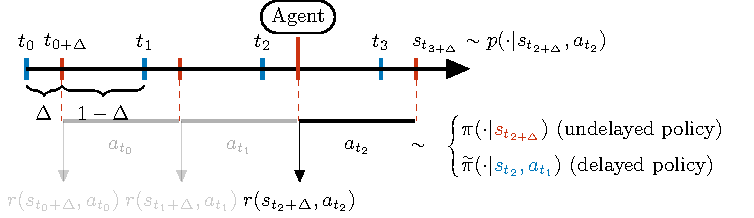
\includegraphics[labelimitation=nonintdelayedmdp]{img/thesis_plots_imitation.pdf}
    \caption{具有非整数动作执行延迟的\gls{dmdp}的表示。}
    \label{fig:non_int_delay_def}
\end{figure}

%=============================================
% 状态相关延迟与动作相关延迟
%---------------------------------------------
\subsection{状态相关延迟与动作相关延迟}
在此设定中，延迟不再独立于智能体的行为。
无论是直接通过动作还是间接通过状态，智能体都可能改变延迟值。
据我们所知，\gls{rl}文献中尚无处理状态相关或动作相关延迟的工作，但实际应用启发这一问题。
例如，使用更复杂的策略选择动作可能获得更优回报，前提是该策略的计算时间合理；当计算时间过大时，使用轻量级策略选择动作则更为合理。
再如，考虑\cite{bouteiller2020reinforcement}中WiFi传输至飞行机器人的设定，延迟很可能取决于机器人与策略计算机之间的距离。

\subsection{关于延迟过程的初始化}
\label{subsec:delay_init}
读者可能会问延迟过程如何初始化。
例如，在状态观测延迟中，如何定义初始状态集合，使得智能体从一开始就有效观测到延迟状态？

这一问题看似浅显，但后文将看到，它可能产生重要的实际影响。
如果仅奖励收集存在延迟，则保持底层\gls{mdp}的初始化方式不会造成问题。
相反，对于动作执行延迟和状态观测延迟，初始化意味着在允许智能体选择任何动作之前，必须以某种方式采样初始的$\delay$个动作。
对于离散或有界动作集，一种任意但合理的采样方案是均匀采样。
这是本文所有实验采用的方法。

注意，取决于初始动作的采样方式以及初始阶段收集的奖励是否计入，智能体的最终回报可能发生显著变化。
举例说明，考虑如下简单\gls{mdp}：奖励等于智能体的速度，且只有一个动作——以固定量"加速"。
在\gls{dmdp}中，初始化意味着"加速"动作在控制权交给智能体之前已经执行了若干次。
这意味着，与初始化速度为0的无延迟智能体相比，延迟智能体在其当前未观测状态中已经累积了速度。
即使初始化阶段的奖励不计入，延迟智能体也以更高的速度起步，从而比无延迟智能体获得更高奖励。
此外，若初始化阶段的奖励计入，则延迟智能体累积更多奖励。
因此，奖励的计入方式可能显著改变延迟智能体相对于无延迟智能体的回报。
我们将这一效应称为延迟初始化偏移（delay initialisation shift）。
